\documentclass[12pt,a4paper]{article}

\usepackage[brazilian]{babel}
\usepackage[utf8]{inputenc}
\usepackage{graphicx}
\usepackage[textsize=tiny]{todonotes}
\usepackage{helvet}
\title{O Sistema \LaTeX}
\author{Henrique Coelho}

\begin{document}
	\maketitle
	\begin{abstract}
		Este artigo é legal e vai servir como exemplo de como utilizar o \LaTeX. Uma ferramenta \textbf{muito divertida} para escrever.
	\end{abstract}
	\tableofcontents
	\section{Introdução}
	A ideia central do \LaTeX\ é distanciar o autor
	o máximo possível da apresentação visual da informação.
	
	Ao invés de trabalhar com ideias visuais, o usuário é
	encorajado a trabalhar com conceitos mais lógicos --- e,
	consequentemente, independente da apresentação --- como capítulos,
	seções, ênfase e tabelas, sem contudo impedir o usuário da
	liberdade de indicar, expressamente, declarações de formatação.
	
	A versão mais recente é a \LaTeXe.
	\subsection{Mundo das Ideias}
	\begin{equation}
		f=\int \frac{sin(x)}{x} dx
	\end{equation}
	
	% Isto é um comentário que não será processado. Ele serve apenas
	% para fazer anotações não incluídas no resultado final. Atenção
	% ao símbolo do comentário: porcentagem (%).
	A seguir, a fórmula das combinações (ver \ref{eq:comb}) como um exemplo simplório
	da capacidade matemática do \LaTeX:
	
	\begin{eqnarray}
		C_k^n &=& \frac{n!}{k!\cdot(n-k)!} \label{eq:comb}
	\end{eqnarray}

	\section{Métodos}
	 Lorem ipsum dolor sit amet, consectetur adipiscing elit. Sed lacinia quis urna sit amet dapibus. Mauris efficitur justo nulla, quis eleifend erat malesuada ut. Vivamus blandit lacus a odio rutrum, non vestibulum mauris consectetur. Nam condimentum pretium luctus. Fusce ac tincidunt purus. Donec iaculis purus turpis. Praesent a placerat tortor. Donec at tempor elit, non consequat mi. Sed ornare dictum nulla. Integer luctus tortor diam, at blandit est dictum quis. Vestibulum sit amet nunc vestibulum, consectetur diam at, molestie neque. Nulla eros arcu, vestibulum id tincidunt vel, bibendum et lacus. Vivamus ac feugiat orci. Quisque ac vehicula odio, eu fringilla sem. Morbi sit amet ante vel diam faucibus maximus sit amet sed diam.\todo{tudo errado, desiste}
	
	\begin{figure}[h!]
		\centering
		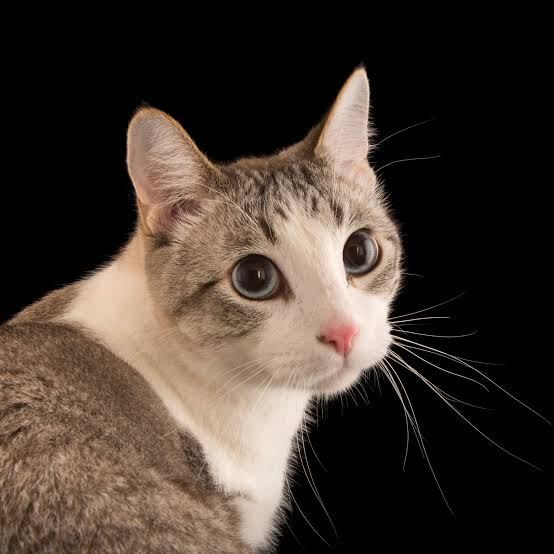
\includegraphics[width=0.7\linewidth]{gato}
		\caption[Gato INSANO]{Talvez isso seja um cachorro.}
		\label{fig:gato}
	\end{figure}
\end{document}
